
% ============================================================
% Representative Market-State Stock Selection
% Draft v9: conference-length version with supplementary diagnostics
% ============================================================

\documentclass[runningheads]{llncs}

\usepackage[T1]{fontenc}
\usepackage{graphicx}
\usepackage{amsmath}
\usepackage{amssymb}
\usepackage{booktabs}
\usepackage{tabularx}
\usepackage{array}
\usepackage{url}
\usepackage{multirow}
\usepackage{algorithm}
\usepackage{algorithmic}
\usepackage{float}

\begin{document}

\title{Representative Market-State Stock Selection: An Exploratory Framework Using PCA-KMeans and Topology-Inspired Benchmarks}
\titlerunning{Representative Market-State Stock Selection}

\author{
Thi Hong Cam Luong\inst{1}\thanks{ORCID: https://orcid.org/0000-0002-9203-0527}
\and
An Vinh Pham\inst{2,3}\thanks{Corresponding author. ORCID: https://orcid.org/0009-0001-0320-5306}
}
\authorrunning{T. H. C. Luong and A. V. Pham}

\institute{
Faculty of Mathematics and Applications, Saigon University,\\
273 An Duong Vuong Street, Cho Quan Ward, Ho Chi Minh City, Vietnam\\
\email{lthcam@sgu.edu.vn}
\and
Faculty of Computer Science and Engineering,\\
Ho Chi Minh City University of Technology (HCMUT),\\
268 Ly Thuong Kiet Street, Ho Chi Minh City, Vietnam\\
\email{vinhpham@hcmut.edu.vn}
\and
Vietnam National University Ho Chi Minh City,\\
Linh Trung Ward, Thu Duc City, Ho Chi Minh City, Vietnam
}

\maketitle

\begin{abstract}
This paper studies representative market-state methods as a stock-selection layer for long-only equity portfolios. At each rebalance date, historical trading days in a rolling lookback window are represented as cross-sectional return vectors. Representative historical states are extracted using a topology-inspired Mapper strategy, Global DBSCAN, or PCA-KMeans; stocks are then ranked by their returns on centroid-nearest representative days and held in equal-weight selected portfolios. The empirical evidence is exploratory. In the main fixed-universe experiment, PCA-KMeans is the strongest representative-state method under the saved balanced-utility ranking, with its best configuration achieving cumulative return of 421.88\%, annualized return of 17.99\%, Daily Sharpe of 0.998, maximum drawdown of -35.51\%, and average one-way rebalancing turnover of 17.23\%. However, this main experiment is subject to fixed-universe and survivorship concerns. A 2020-start public reconstructed S\&P 500 robustness test gives mixed results and does not support market-outperformance claims, while a 2023-onward regime-sensitivity diagnostic is more favorable but still dominated by the capitalization-weighted S\&P 500. Bootstrap intervals are wide and pairwise confidence intervals contain zero. Overall, the results are consistent with possible regime-dependent usefulness of representative-state stock selection, not with proven alpha or a complete trading system.

\keywords{Representative market states \and Stock selection \and PCA-KMeans \and Mapper \and Topological Data Analysis \and Clustering \and Quantitative finance}
\end{abstract}

\section{Introduction}

Equity stock selection is difficult because returns are noisy, high-dimensional, and non-stationary. A stock's realized performance depends not only on its own characteristics, but also on time-varying market states, sector rotations, broad risk appetite, liquidity conditions, and changing common-factor exposures. Classical portfolio theory and performance evaluation already emphasize the importance of portfolio-level risk and risk-adjusted evaluation~\cite{markowitz1952,sharpe1966}. This motivates methods that do not treat each stock's time series independently. Instead, this paper asks whether the geometry of recent market states can be converted into a useful cross-sectional stock-selection signal.

The framework treats each historical trading day in a rolling lookback window as a market-state observation represented by a vector of stock returns. A representative-date extraction method identifies a small number of historical days that summarize important regions of the recent market-state space. Stocks are then ranked by their realized cross-sectional returns on those representative days, and the strongest stocks are selected into a long-only, fully invested, equal-weight portfolio until the next rebalance.

The selection rule is based on a deliberately simple empirical hypothesis: if representative recent market states capture recurring or economically relevant regions of market behavior, then stocks that performed relatively well on those representative states may proxy for resilience or relative strength under related conditions. This hypothesis is tested empirically in the saved backtests; it is not assumed to be a structural asset-pricing law.

The original conceptual motivation comes from Topological Data Analysis (TDA), especially Mapper~\cite{singh2007,carlsson2009,edelsbrunner2010}. Mapper is useful because it provides a topology-inspired way to summarize the structure of high-dimensional data through a graph of local clusters. Prior work has also explored TDA-based diagnostics for financial time series and market stress~\cite{gidea2018,gidea2020crypto}. In this study, however, the empirical claim is not that Mapper is superior. Mapper is retained as the topology-inspired conceptual origin and benchmark, while PCA-KMeans is the strongest representative-state method under the saved balanced-ranking criteria in the main fixed-universe experiment and in the 2023-onward regime-sensitivity diagnostic. This statement refers to the saved composite ranking, not to dominance on every individual return-side metric.

The contribution is therefore deliberately modest. The paper proposes and evaluates a representative market-state stock-selection layer. It compares Mapper, Global DBSCAN, and PCA-KMeans representative-date extraction; benchmarks the strongest configurations against Equal Weight, the S\&P 500, cross-sectional momentum~\cite{jegadeesh1993}, and random representative-date trials; and adds a public 2020-start universe robustness test plus a 2023-onward regime-sensitivity diagnostic. The paper does not claim market timing, dynamic risk management, statistical alpha, or direct investability.

This distinction is important. The tested portfolios are long-only and fully invested. They contain no cash allocation, no hedging, no volatility targeting, no stop loss, and no explicit regime-switching rule. As a result, even a useful selection signal can still experience broad equity-market drawdowns. The appropriate reading is that the evidence is consistent with the possibility of a useful cross-sectional stock-selection signal within a long-only framework, especially in supportive regimes. They are not, by themselves, a risk-management system.

\section{Methodology}

\subsection{Return Definition and Lookback Matrix}

Let $P_{i,t}$ denote the adjusted close price of stock $i$ on trading day $t$. The daily simple return is
\begin{equation}
R_{i,t} = \frac{P_{i,t}}{P_{i,t-1}} - 1.
\end{equation}
At each rebalance date $\tau$, the method uses a rolling lookback window of $W=504$ trading days. The lookback matrix is
\begin{equation}
X_{\tau} \in \mathbb{R}^{W \times N},
\end{equation}
where each row is a historical trading day and each column is a stock. Columns are standardized stock by stock within the lookback window. Stocks with incomplete return histories in the lookback window are excluded from that rebalance calculation, avoiding forward-fill or backward-fill assumptions.

\subsection{Representative-Date Extraction}

The method extracts $k=3$ representative historical trading days from the standardized lookback matrix. A representative day is an observed trading day nearest to a node or cluster centroid. This centroid-nearest day is medoid-like, but it should not be confused with a classical pairwise-distance medoid unless the implementation explicitly computes pairwise medoids. Its role is to translate an abstract market-state region into an actual trading day with a realized cross-section of stock returns.

For each representative day $d$, stocks are ranked by $R_{i,d}$, their same-day cross-sectional return. The top $l$ fraction is selected, where $l \in \{0.20,0.30,0.40\}$. If $S_{\tau}^{(j)}$ denotes the selected stock set from representative day $j$, the rebalance stock set is
\begin{equation}
S_{\tau}=\bigcup_{j=1}^{3}S_{\tau}^{(j)}.
\end{equation}
The portfolio is equal-weight across $S_{\tau}$ and held until the next rebalance date.

\subsection{Mapper, Global DBSCAN, and PCA-KMeans}

The Mapper strategy follows the standard Mapper construction and related software practice~\cite{singh2007,carlsson2009,vanveen2019}. It applies PCA~\cite{jolliffe2002} to the standardized lookback matrix and uses the first principal-component score as the Mapper lens. The lens is covered by overlapping intervals, local DBSCAN clustering~\cite{ester1996} is performed inside intervals, and the largest valid Mapper nodes are used to obtain centroid-nearest representative days. Mapper is topology-inspired and is the conceptual origin of the framework.

The Global DBSCAN benchmark applies PCA and then clusters the market-state observations with DBSCAN globally in PCA space. Its interpretation is more fragile because DBSCAN can produce too few valid clusters under fixed parameters. When there are too few valid clusters, fallback handling is used, so the method is best read as a DBSCAN-anchored representative-date benchmark rather than a pure density-clustering result.

The PCA-KMeans strategy applies PCA and then KMeans~\cite{macqueen1967} with $k=3$ clusters. For each cluster, the observed day nearest to the cluster centroid becomes the representative day. This method is simple, stable, and empirically strong under the saved balanced-ranking criteria. In some subsamples, other methods can have higher return-side point estimates, so PCA-KMeans should not be read as uniformly dominant on every metric.

\subsection{Portfolio Construction and Turnover}

All tested representative-state portfolios are long-only, fully invested, and equal-weight after selection. The experiments do not use leverage, short positions, mean-variance optimization, sector neutrality, cash allocation, hedging, volatility targeting, or market-regime switching.

Average Turnover means average one-way rebalancing turnover, not average daily turnover. At each rebalance date,
\begin{equation}
\text{Turnover}_{\tau}=\frac{1}{2}\sum_i\left|w^{new}_{i,\tau}-w^{old}_{i,\tau}\right|,
\end{equation}
where $w^{old}_{i,\tau}$ is the pre-rebalance actual weight after price drift and $w^{new}_{i,\tau}$ is the new target weight. The transaction-cost convention in the saved experiments is simplified and should not be interpreted as a full execution-cost model.

\begin{algorithm}
\caption{Representative Market-State Stock Selection at Rebalance Date $\tau$}
\label{alg:representative_market_state}
\begin{algorithmic}[1]
\REQUIRE Return panel $R$, rebalance date $\tau$, lookback $W$, representative count $k$, selection fraction $l$, extraction method $m$
\STATE Construct $X_{\tau}$ from trading days $[\tau-W,\tau-1]$.
\STATE Remove stocks with incomplete lookback histories and standardize columns.
\STATE Apply method $m$ to obtain representative nodes or clusters. If fewer than $k$ valid nodes or clusters are available, apply the method-specific fallback policy documented in the supplementary replication package.
\STATE Select the centroid-nearest observed trading day from each valid node or cluster.
\STATE Rank stocks by same-day cross-sectional return on each representative day.
\STATE Select the top $l$ fraction from each representative day and form their union.
\STATE Hold an equal-weight long-only portfolio until the next rebalance.
\STATE Record NAV, returns, rebalancing turnover, selected-stock count, and diagnostics.
\end{algorithmic}
\end{algorithm}

\section{Experimental Design}

The experiments use saved artifacts from the project outputs. Standard PCA, KMeans, and DBSCAN implementations are consistent with common machine-learning tooling such as scikit-learn~\cite{pedregosa2011}. The core parameters are $W=504$, $k=3$, rebalance frequencies $h\in\{21,42,63\}$ trading days, and selection fractions $l\in\{0.20,0.30,0.40\}$. The main metrics are cumulative return, annualized return, Daily Sharpe, daily maximum drawdown, average one-way rebalancing turnover, and average number of selected stocks. Throughout the paper, Daily Sharpe denotes the annualized Sharpe ratio computed from daily after-cost portfolio returns,
\[
\mathrm{Sharpe}_{\mathrm{daily}}=\frac{\bar r_d}{s_d}\sqrt{252},
\]
where $\bar r_d$ and $s_d$ are the sample mean and sample standard deviation of daily returns. The label is retained to emphasize that the statistic is estimated from daily returns rather than from monthly or annual observations. Bootstrap uncertainty diagnostics follow the moving-block bootstrap idea of resampling dependent time-series data~\cite{kunsch1989}. The implementation parameters recovered from the supplied notebooks, metadata files, and saved computational artifacts are summarized below and documented in full in the supplementary replication package. These details are included to make the exploratory backtests auditable; stronger practical claims would still require cleaner point-in-time data and pre-specified validation rules.

The saved artifacts use two different composite-ranking conventions. The Step 4 artifact reports a normalized balanced-utility score, where larger values are better. Let $r_m(c)$ be the within-experiment rank of configuration $c$ on metric $m$ after applying the favorable direction: annualized return and Daily Sharpe are ranked high-to-low, daily maximum drawdown is ranked with less severe drawdown favored, and average one-way rebalancing turnover is ranked low-to-high. For a ranking population of size $N$, the Step 4 normalized rank score is
\[
q_m(c)=\frac{N-r_m(c)+1}{N},
\]
and the saved Step 4 balanced utility is
\[
U(c)=0.35q_{\mathrm{Ann}}(c)+0.35q_{\mathrm{Sharpe}}(c)+0.20q_{\mathrm{MDD}}(c)+0.10q_{\mathrm{Turnover}}(c).
\]
Thus larger $U(c)$ indicates better composite performance. The Step 5 and Step 5B artifacts instead report a weighted rank-sum score,
\[
RS(c)=0.35r_{\mathrm{Ann}}(c)+0.35r_{\mathrm{Sharpe}}(c)+0.20r_{\mathrm{MDD}}(c)+0.10r_{\mathrm{Turnover}}(c),
\]
so smaller values indicate better composite trade-offs. The composite rankings do not use cumulative return directly; cumulative return is reported as a descriptive performance metric. Because the two artifacts use different score directions, this paper does not compare Utility and Rank Sum values across experiments. They are used only to reproduce and summarize the saved within-experiment rankings; they are not independent statistical tests and should not be interpreted as $p$-values, confidence measures, or evidence of statistical superiority.


The core implementation settings are as follows. The experiments use daily simple adjusted-close returns, lookback $W=504$ trading days, representative count $k=3$, rebalance frequencies $h\in\{21,42,63\}$, and selection fractions $l\in\{0.20,0.30,0.40\}$. Portfolios are long-only and equal-weight after selection, with initial NAV 1,000,000 and transaction cost $0.001\times$ NAV $\times$ one-way rebalancing turnover. PCA-based clustering uses up to 10 components; PCA-KMeans uses $k=3$, random state 42, and \texttt{n\_init}=10. Global DBSCAN uses minimum samples 5 and an epsilon based on the 70th percentile of nearest-neighbor distances. The main fixed-universe Mapper uses the deterministic adaptive grid and fallback policy provided in the replication package; the 2020-start and 2023-onward diagnostics use 10 cover intervals, 30\% overlap, local DBSCAN, and minimum samples 5. Random-date diagnostics use 100 trials with seed base 42. Bootstrap diagnostics use a moving-block bootstrap with 1,000 samples, block length 21 trading days, and seed base 42. The supplementary replication package provides the full parameter manifest, notebooks, diagnostic CSVs, checksums, requirements file, and the recovered main-universe returns matrix used for supplementary diagnostics.


The main fixed-universe experiment uses a current/recent large-cap U.S. equity universe. This is useful for controlled method comparison but is not a survivorship-free point-in-time S\&P 500 backtest. Its strongest use is signal discovery: whether representative market-state extraction is associated with useful cross-sectional stock-selection information under a consistent large-cap universe.

Step 4 adds robustness around the main fixed-universe experiment. Step 4 Exp. 1 reports the full balanced-utility ranking. Step 4 Exp. 2 adds cross-sectional momentum benchmarks. Step 4 Exp. 3 adds corrected random representative-date trials. In response to audit concerns, this draft also adds two supplementary diagnostics on the recovered main-universe return matrix: a $k$-ablation for PCA-KMeans at $h=21,l=20\%$ and a simple forward-split diagnostic that calibrates PCA-KMeans hyperparameters on the early part of the sample and evaluates the chosen configuration from 2019 onward. These diagnostics are not treated as substitutes for a full pre-registered walk-forward study.

Step 5 uses a public reconstructed S\&P 500 constituent list fixed around the start of 2020 and evaluates performance from 2020-01-02 to 2025-12-31. This is not a fully survivorship-free CRSP/Compustat/WRDS point-in-time backtest. It is a start-of-period fixed-universe robustness test that reduces the most direct end-of-sample universe-selection concern while retaining public-data limitations.

Step 5B reuses the 2020-start universe and data, but evaluates from 2023 onward. This is a post-hoc exploratory regime-sensitivity diagnostic, not a replacement for Step 5 and not a confirmatory out-of-sample test. Its purpose is to check whether the stock-selection signal appears more visible after the difficult 2022 bear/rate-hike regime and during the subsequent recovery. Results from Step 5 and Step 5B must be read together.

\section{Results}

\subsection{Main Fixed-Universe Balanced-Utility Ranking}

Table~\ref{tab:step4_top_ranking} reports the top twelve rows from the full Step 4 balanced-utility ranking. The complete ranking contains 33 rows in the saved artifact \texttt{step4\_full\_balanced\_score\_ranking.csv}. PCA-KMeans with $h=21$ and $l=20\%$ ranks first under this saved utility criterion, followed by another PCA-KMeans configuration and then Mapper with $h=21$ and $l=20\%$. The result supports a representative-state framing, but not a Mapper-superiority claim.

\begin{table}[t]
\centering
\caption{Step 4 main fixed-universe top balanced-utility configurations; larger Utility is better.}
\label{tab:step4_top_ranking}
\scriptsize
\setlength{\tabcolsep}{2.5pt}
\begin{tabular}{rllrrrrrrr}
\toprule
Rank & Method & $h$ & $l$ & Cum. & Ann. & Sharpe & MDD & Turnover & Utility \\
\midrule
1 & PCA-KMeans & 21 & 20\% & 421.88\% & 17.99\% & 0.998 & -35.51\% & 17.23\% & 0.9091 \\
2 & PCA-KMeans & 21 & 30\% & 384.01\% & 17.10\% & 0.968 & -35.45\% & 12.93\% & 0.8606 \\
3 & Mapper & 21 & 20\% & 401.27\% & 17.51\% & 0.970 & -35.84\% & 16.79\% & 0.8515 \\
4 & PCA-KMeans & 42 & 20\% & 415.23\% & 17.84\% & 0.991 & -35.79\% & 23.31\% & 0.8515 \\
5 & PCA-KMeans & 42 & 30\% & 382.79\% & 17.07\% & 0.966 & -35.73\% & 17.55\% & 0.7939 \\
6 & PCA-KMeans & 21 & 40\% & 378.38\% & 16.97\% & 0.963 & -36.15\% & 9.66\% & 0.7530 \\
7 & Mapper & 42 & 20\% & 388.44\% & 17.21\% & 0.961 & -36.12\% & 25.72\% & 0.7348 \\
8 & Mapper & 63 & 20\% & 381.98\% & 17.05\% & 0.947 & -35.34\% & 28.78\% & 0.7182 \\
9 & PCA-KMeans & 63 & 20\% & 394.90\% & 17.36\% & 0.965 & -36.81\% & 29.85\% & 0.6970 \\
10 & PCA-KMeans & 42 & 40\% & 372.82\% & 16.83\% & 0.956 & -36.35\% & 12.95\% & 0.6924 \\
11 & Global DBSCAN & 21 & 20\% & 379.06\% & 16.98\% & 0.944 & -36.62\% & 15.14\% & 0.6606 \\
12 & Global DBSCAN & 21 & 30\% & 369.55\% & 16.75\% & 0.943 & -36.43\% & 12.00\% & 0.6439 \\
\bottomrule
\end{tabular}
\end{table}

The best PCA-KMeans configuration obtains cumulative return of 421.88\%, annualized return of 17.99\%, Daily Sharpe of 0.998, daily maximum drawdown of -35.51\%, average one-way rebalancing turnover of 17.23\%, and an average of 175.2 stocks. These are point estimates in a fixed-universe exploratory experiment. They should not be interpreted as proof of alpha or as evidence of direct investability.

\subsection{Momentum Benchmark}

The Step 4 momentum artifact compares the strongest representative-state configurations with benchmark rows and the best momentum configurations. PCA-KMeans has stronger point estimates than Momentum 21D and Momentum 63D. Momentum 126D is competitive, with annualized return of 17.27\% and Daily Sharpe of 0.924, but its turnover is much higher than PCA-KMeans: 46.99\% versus 17.23\% average one-way rebalancing turnover. This supports the interpretation that representative-state selection is not simply a high-turnover trailing-return rule in the main fixed-universe setting.


The detailed benchmark table is moved to the supplementary replication package for page economy. In the saved Step 4 comparison, PCA-KMeans $h=21,l=20\%$ obtains 421.88\% cumulative return, 17.99\% annualized return, Daily Sharpe 0.998, MDD -35.51\%, and turnover 17.23\%. Momentum 126D is the closest momentum benchmark, with 390.98\% cumulative return, 17.27\% annualized return, Daily Sharpe 0.924, MDD -36.48\%, and turnover 46.99\%. Equal Weight Universe obtains 348.45\% cumulative return, 16.21\% annualized return, Daily Sharpe 0.916, and turnover 5.76\%, while the S\&P 500 obtains 242.64\% cumulative return and Daily Sharpe 0.773 over the same saved main fixed-universe comparison.


\subsection{Random Representative-Date Trials}

The corrected Step 4 random-date trials provide a baseline in which representative days are randomized while portfolio construction remains comparable. For PCA-KMeans $h=21,l=20\%$, annualized return is at the 97th percentile of the corrected random-date distribution, Daily Sharpe lies at the upper end of the corrected random-date distribution, daily maximum drawdown is at the 97th percentile, and turnover lies near the lower tail of the random-date distribution under the saved percentile convention. The mean random-date annualized return is 16.19\%, mean Daily Sharpe is 0.889, mean daily maximum drawdown is -37.58\%, and mean turnover is 50.45\%.

These results are favorable for the fixed-universe signal-discovery interpretation. They do not by themselves establish statistical superiority or market outperformance, but they are consistent with the representative-date extraction rule adding structure beyond arbitrary historical-date selection.


\subsection{Supplementary $k$-Ablation and Forward-Split Diagnostics}

Two audit-motivated diagnostics were added to address sensitivity to the representative count and to reduce the concern that the selected PCA-KMeans configuration is purely a full-sample artifact. Full diagnostic tables are provided in the supplementary replication package. First, a PCA-KMeans $k$-ablation on the recovered main fixed-universe return matrix with $h=21$ and $l=20\%$ compares $k\in\{1,2,3,4,5\}$. In that diagnostic, $k=3$ has the strongest annualized return, Sharpe, and maximum-drawdown profile among the tested values, with cumulative return of 409.10\%, annualized return of 17.73\%, Daily Sharpe of 0.991, maximum drawdown of -35.54\%, and turnover of 17.08\%. These values use the recovered return matrix included in the replication package and are intended as supplementary diagnostics rather than byte-for-byte reproductions of the saved Step 4 ranking artifact; this explains the small difference from the corresponding saved Step 4 row in Table~\ref{tab:step4_top_ranking}.

Second, a simple forward-split diagnostic evaluates whether the selected configuration is entirely driven by full-sample selection. A calibration grid over PCA-KMeans configurations with $k=3$, $h\in\{21,42,63\}$, and $l\in\{20\%,30\%,40\%\}$ was evaluated on the early recovered sample ending 2018-12-31. The same balanced-utility criterion selected $h=21,l=20\%$. Holding this configuration fixed from 2019 onward gives cumulative return of 226.51\%, annualized return of 18.47\%, Daily Sharpe of 0.950, maximum drawdown of -36.16\%, and average turnover of 18.37\%. This diagnostic does not remove the fixed-universe concern and is not a substitute for a fully pre-specified walk-forward study, but it weakens the claim that the reported main configuration is purely a full-sample selection artifact.

\subsection{2020-Start Universe Robustness}

Table~\ref{tab:step5_2020} summarizes the top rows from the 2020-start fixed-universe robustness test. The ranking is mixed and weaker for the representative-state methods. The S\&P 500 index benchmark ranks first in the balanced rank-sum table, with cumulative return of 111.88\%, annualized return of 13.37\%, Daily Sharpe of 0.705, and daily maximum drawdown of -33.92\%. The best PCA-KMeans representative-state row ranks fifth, with cumulative return of 95.89\%, annualized return of 11.89\%, Daily Sharpe of 0.623, daily maximum drawdown of -38.97\%, and turnover of 18.27\%.

\begin{table}[t]
\centering
\caption{Step 5 2020-start fixed-universe robustness: selected balanced rank-sum rows; smaller Rank Sum is better. Repeated S\&P 500 rows are retained because the saved artifact records the index benchmark under each rebalance-frequency label.}
\label{tab:step5_2020}
\scriptsize
\setlength{\tabcolsep}{2.3pt}
\begin{tabular}{rllrrrrrrr}
\toprule
Rank & Method & $h$ & $l$ & Cum. & Ann. & Sharpe & MDD & Turnover & Rank Sum \\
\midrule
1 & S\&P 500 Index Benchmark & 21 & -- & 111.88\% & 13.37\% & 0.705 & -33.92\% & 0.00\% & 2.00 \\
4 & Equal Weight Universe & 63 & -- & 99.44\% & 12.23\% & 0.635 & -39.37\% & 7.20\% & 7.20 \\
5 & PCA-KMeans & 63 & 40\% & 95.89\% & 11.89\% & 0.623 & -38.97\% & 18.27\% & 8.55 \\
6 & PCA-KMeans & 21 & 20\% & 96.09\% & 11.91\% & 0.614 & -39.02\% & 23.61\% & 10.30 \\
7 & PCA-KMeans & 21 & 40\% & 97.55\% & 12.05\% & 0.628 & -39.68\% & 12.04\% & 10.60 \\
10 & Mapper & 63 & 40\% & 90.10\% & 11.33\% & 0.599 & -38.65\% & 13.81\% & 12.50 \\
\bottomrule
\end{tabular}
\end{table}

The Step 5 momentum comparison also does not support an unconditional market-beating claim. In the top comparison rows, Momentum 21D with $h=42,l=40\%$ has annualized return of 13.50\% and Daily Sharpe of 0.716, whereas the best PCA-KMeans row has annualized return of 11.89\% and Daily Sharpe of 0.623. The representative-state method remains a stock-selection signal candidate, but this robustness layer shows that stock selection alone does not solve adverse market regimes and does not automatically beat simple benchmarks.

\subsection{2023-Onward Regime-Sensitivity Diagnostic}

Table~\ref{tab:step5b_2023} reports the top rows from the 2023-onward regime-sensitivity diagnostic. The S\&P 500 remains strongest in this period, with cumulative return of 78.29\%, annualized return of 21.38\%, and Daily Sharpe of 1.362. This capitalization-weighted benchmark comparison limits the strength of any practical performance claim. At the same time, it clarifies that an equal-weight selected-stock basket is being evaluated under a different weighting scheme, not under capitalization weighting.

Within the long-only stock-selection setting, PCA-KMeans becomes more favorable under the saved balanced rank-sum criterion. PCA-KMeans $h=21,l=40\%$ obtains cumulative return of 48.57\%, annualized return of 14.19\%, Daily Sharpe of 0.955, daily maximum drawdown of -18.75\%, and average turnover of 14.94\%. Equal Weight obtains annualized return of 13.89\% and Daily Sharpe of 0.945. Momentum 126D obtains cumulative return of 48.06\%, annualized return of 14.06\%, Daily Sharpe of 0.959, and daily maximum drawdown of -19.30\%, but its turnover is 42.45\%, substantially higher than PCA-KMeans.

\begin{table}[t]
\centering
\caption{Step 5B 2023-onward regime sensitivity: selected balanced rank-sum rows; smaller Rank Sum is better. Repeated S\&P 500 rows are retained because the saved artifact records the index benchmark under each rebalance-frequency label.}
\label{tab:step5b_2023}
\scriptsize
\setlength{\tabcolsep}{2.3pt}
\begin{tabular}{rllrrrrrrr}
\toprule
Rank & Method & $h$ & $l$ & Cum. & Ann. & Sharpe & MDD & Turnover & Rank Sum \\
\midrule
1 & S\&P 500 Index Benchmark & 21 & -- & 78.29\% & 21.38\% & 1.362 & -18.90\% & 0.00\% & 3.00 \\
4 & PCA-KMeans & 21 & 40\% & 48.57\% & 14.19\% & 0.955 & -18.75\% & 14.94\% & 6.60 \\
5 & Global DBSCAN & 63 & 20\% & 49.65\% & 14.46\% & 0.962 & -18.62\% & 37.97\% & 7.90 \\
6 & Equal Weight Universe & 63 & -- & 47.40\% & 13.89\% & 0.945 & -18.57\% & 8.91\% & 8.25 \\
7 & Global DBSCAN & 42 & 20\% & 55.00\% & 15.82\% & 1.017 & -19.37\% & 32.71\% & 8.30 \\
\bottomrule
\end{tabular}
\end{table}

It is important that PCA-KMeans is not uniformly best on every individual metric in this diagnostic. For example, some Global DBSCAN configurations have higher return-side point estimates than the top-ranked PCA-KMeans row. PCA-KMeans is described as stronger here because the saved rank-sum criterion jointly accounts for return, Sharpe, drawdown, and turnover trade-offs.

\begin{figure}[t]
\centering
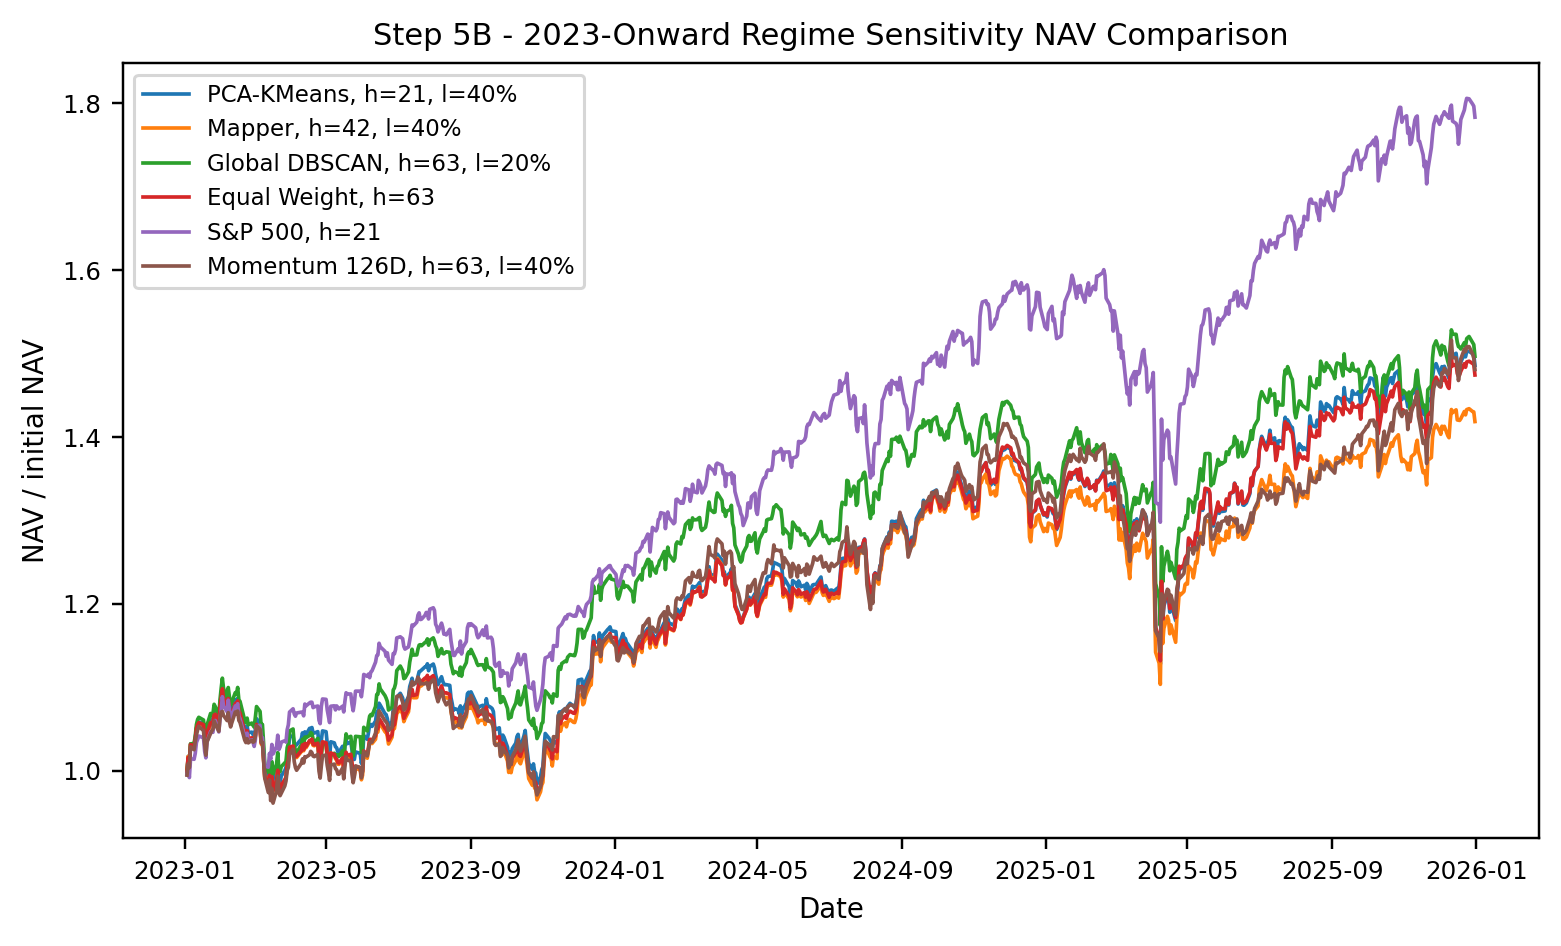
\includegraphics[width=0.72\linewidth]{figures/nav_comparison_2023_regime_sensitivity.png}
\caption{NAV comparison for the 2023-onward regime-sensitivity diagnostic from the saved Step 5B artifact.}
\label{fig:nav_2023}
\end{figure}

The 2023-onward random-date diagnostics are also favorable for the representative-state interpretation. Random-date trials have mean annualized return of 13.27\%, mean Daily Sharpe of 0.863, mean daily maximum drawdown of -20.60\%, and mean turnover of 51.37\%. PCA-KMeans has similar or better point estimates on return and Sharpe, slightly better drawdown, and far lower turnover. This supports the exploratory interpretation that representative-state selection may encode a useful stock-selection signal in a supportive long-only regime.

\subsection{Bootstrap Uncertainty}

Bootstrap uncertainty remains wide. In the 2020-start robustness test, all 12 saved pairwise 95\% confidence intervals contain zero. In the 2023-onward regime-sensitivity diagnostic, all 15 saved pairwise 95\% confidence intervals also contain zero. Therefore, the paper should not claim statistical superiority.


For compactness, the detailed Daily Sharpe bootstrap interval table is moved to the supplementary replication package. The saved intervals are wide. For example, the 2020-start PCA-KMeans row has 95\% Daily Sharpe CI $[-0.078,1.457]$, while the 2023-onward PCA-KMeans row has 95\% Daily Sharpe CI $[-0.120,1.981]$.


Detailed Daily Sharpe intervals are moved to the supplementary replication package for compactness; the saved bootstrap artifacts also contain annualized-return and maximum-drawdown intervals. The point estimates are favorable in selected settings, especially for PCA-KMeans in the main fixed-universe experiment and in the 2023-onward diagnostic. However, bootstrap intervals remain wide and do not support a statistical superiority claim. The appropriate conclusion is evidence consistent with possible regime-dependent usefulness as a stock-selection layer, not proven alpha.

\section{Discussion}

The evidence supports a careful interpretation. Representative market states can provide a structured way to transform recent market-state geometry into a cross-sectional stock-selection signal. In the main fixed-universe experiment, PCA-KMeans performs best among tested representative-state methods and compares favorably with corrected random-date trials. In the 2023-onward diagnostic, PCA-KMeans is close to Equal Weight and the best momentum benchmark in point estimates while using substantially less turnover than the best momentum benchmark. These observations are consistent with the possibility that representative-state selection encodes a useful cross-sectional signal in some long-only settings.

The 2020-start robustness test is equally important. It shows mixed and weaker results relative to the S\&P 500, Equal Weight, and the best momentum benchmark. This weakens the practical performance claim and indicates that the signal, if present, is not sufficient without a separate market-exposure control layer. In adverse regimes, such as the 2022 bear/rate-hike environment embedded in the Step 5 period, a fully invested long-only portfolio can suffer from broad market exposure even when its stock-selection signal is informative.

The S\&P 500's dominance in the 2023-onward diagnostic limits the strength of any practical performance claim. At the same time, it does not directly test the same object as the selected portfolios: the S\&P 500 is capitalization-weighted, whereas the representative-state portfolios are equal-weight selected-stock baskets. The comparison therefore shows that the proposed stock-selection layer does not dominate a capitalization-weighted benchmark in this regime, while leaving open the narrower question of whether the selected equal-weight baskets contain useful cross-sectional information.

Mapper remains conceptually valuable but not empirically dominant in these outputs. It motivates the topology-inspired view of market-state structure, while PCA-KMeans provides the strongest representative-date extraction method under the saved composite-ranking criteria in the current experiments. This is a criterion-dependent statement, not a claim of uniform dominance on every individual metric. Global DBSCAN remains a useful benchmark but requires caution because its clustering behavior and fallback handling can affect interpretation.

\section{Limitations}

The study has important limitations. First, the main experiment uses a fixed large-cap universe and is subject to survivorship and ex-post universe-construction concerns. Second, the 2020-start universe is a public reconstructed start-of-period universe, not an official CRSP/WRDS point-in-time index-membership backtest with delisting-adjusted returns. Third, the data source is based on public/yfinance-derived adjusted prices, which can contain data-quality limitations. Fourth, the paper does not yet include factor-model attribution, Fama--French regression~\cite{fama1993}, sector-neutral alpha tests, or comparisons against standard value, quality, low-volatility, and size factor portfolios.

Fifth, the portfolios are long-only, equal-weight, and fully invested. They have no dynamic capital allocation, no cash allocation, no hedging, no volatility targeting, no stop-loss rule, no drawdown-control overlay, and no market-regime model. Sixth, the transaction-cost convention is simplified and does not model bid--ask spreads, market impact, liquidity, tax, borrow, or capacity constraints. Seventh, bootstrap uncertainty is wide and pairwise differences do not support statistical superiority. Eighth, the newly added $k$-ablation and forward-split diagnostics are useful sanity checks, but they are still based on the same public fixed-universe data and are not a substitute for a fully pre-specified walk-forward study.

Taken together, the current empirical results should be viewed as hypothesis-generating rather than confirmatory.

\section{Future Work}

Future work should add a true point-in-time historical universe using CRSP/Compustat or WRDS-style membership and delisting-adjusted data. It should also add factor-model attribution, sector-neutral tests, Fama--French and momentum-factor regressions, and broader comparisons with factor portfolios~\cite{fama1993}.

A second direction is risk management. The current paper intentionally isolates stock selection. Future implementations could add dynamic capital allocation, market-regime detection, trend filters, volatility targeting, cash allocation, hedging, and drawdown-aware exposure scaling. These extensions would test whether representative-state stock selection can be combined with a separate market-exposure control layer.

A third direction is validation design. The framework should be tested with fully pre-specified walk-forward model selection, larger holdout periods, broader $k$- and lookback-window ablations, alternative representative-date definitions, alternative scoring rules, shrinkage-based covariance variants~\cite{ledoit2004}, transaction-cost sensitivity, sector constraints, liquidity filters, and larger out-of-sample studies. Hierarchical or diversified portfolio-construction ideas could also be compared in later extensions~\cite{lopezdeprado2016}. These experiments are necessary before making stronger practical or investability claims.

\section{Conclusion}

This paper evaluates representative market-state methods as a stock-selection layer for long-only equity portfolios. Historical trading days are represented as cross-sectional return vectors, representative days are extracted using Mapper, Global DBSCAN, or PCA-KMeans, and stocks that performed strongly on centroid-nearest representative days are selected into equal-weight portfolios.

The evidence is consistent with the possibility that representative-state methods may encode useful cross-sectional stock-selection information, especially in supportive long-only regimes. PCA-KMeans is the strongest representative-state method under the saved balanced-ranking criteria in the main fixed-universe experiment and remains favorable in the post-hoc 2023-onward regime-sensitivity diagnostic. However, the 2020-start robustness test is mixed and weaker against the S\&P 500, Equal Weight, and momentum. Bootstrap intervals are wide and pairwise differences do not support statistical superiority.

The framework should therefore be read as exploratory stock-selection research, not as proof of alpha, not as a market-beating system, and not as a complete trading strategy. Dynamic capital allocation, market-regime reading, volatility targeting, hedging, cash allocation, factor-neutral testing, and point-in-time data validation are natural future-work extensions.

\section*{Acknowledgment}

The first author acknowledges Saigon University for supporting this study. The corresponding author acknowledges Ho Chi Minh City University of Technology (HCMUT), VNU-HCM, for supporting this study.

\paragraph{Data and code availability.} A supplementary replication package has been prepared with the supplied Step 4, Step 5, and Step 5B notebooks, diagnostic CSV files, the recovered returns matrix used in the supplementary diagnostics, checksums, and a reference requirements file. Because yfinance adjusted prices can change retroactively, exact replication should use the saved matrices and artifacts in the package rather than relying only on live re-downloads.

\paragraph{Conflicts of interest.} The authors declare no conflicts of interest.

\begin{thebibliography}{99}

\bibitem{markowitz1952}
Markowitz, H.: Portfolio selection. Journal of Finance 7(1), 77--91 (1952)

\bibitem{sharpe1966}
Sharpe, W.F.: Mutual fund performance. Journal of Business 39(1), 119--138 (1966)

\bibitem{jolliffe2002}
Jolliffe, I.T.: Principal Component Analysis. Springer, New York (2002)

\bibitem{macqueen1967}
MacQueen, J.: Some methods for classification and analysis of multivariate observations. In: Proceedings of the Fifth Berkeley Symposium on Mathematical Statistics and Probability, pp. 281--297 (1967)

\bibitem{ester1996}
Ester, M., Kriegel, H.-P., Sander, J., Xu, X.: A density-based algorithm for discovering clusters in large spatial databases with noise. In: Proceedings of the Second International Conference on Knowledge Discovery and Data Mining, pp. 226--231 (1996)

\bibitem{singh2007}
Singh, G., M\'emoli, F., Carlsson, G.: Topological methods for the analysis of high dimensional data sets and 3D object recognition. In: Eurographics Symposium on Point-Based Graphics, pp. 91--100 (2007). \doi{10.2312/SPBG/SPBG07/091-100}

\bibitem{carlsson2009}
Carlsson, G.: Topology and data. Bulletin of the American Mathematical Society 46(2), 255--308 (2009)

\bibitem{edelsbrunner2010}
Edelsbrunner, H., Harer, J.: Computational Topology: An Introduction. American Mathematical Society (2010)

\bibitem{jegadeesh1993}
Jegadeesh, N., Titman, S.: Returns to buying winners and selling losers: implications for stock market efficiency. Journal of Finance 48(1), 65--91 (1993)

\bibitem{fama1993}
Fama, E.F., French, K.R.: Common risk factors in the returns on stocks and bonds. Journal of Financial Economics 33(1), 3--56 (1993)

\bibitem{ledoit2004}
Ledoit, O., Wolf, M.: Honey, I shrunk the sample covariance matrix. Journal of Portfolio Management 30(4), 110--119 (2004)

\bibitem{vanveen2019}
van Veen, H.J., Saul, N., Eargle, D., Mangham, S.W.: Kepler Mapper: A flexible Python implementation of the Mapper algorithm. Journal of Open Source Software 4(42), 1315 (2019). \doi{10.21105/joss.01315}

\bibitem{pedregosa2011}
Pedregosa, F., Varoquaux, G., Gramfort, A., Michel, V., Thirion, B., Grisel, O., Blondel, M., Prettenhofer, P., Weiss, R., Dubourg, V., et al.: Scikit-learn: Machine Learning in Python. Journal of Machine Learning Research 12, 2825--2830 (2011)

\bibitem{gidea2018}
Gidea, M., Katz, Y.: Topological data analysis of financial time series: Landscapes of crashes. Physica A: Statistical Mechanics and its Applications 491, 820--834 (2018). \doi{10.1016/j.physa.2017.09.028}

\bibitem{gidea2020crypto}
Gidea, M., Goldsmith, D., Katz, Y., Roldan, P., Shmalo, Y.: Topological recognition of critical transitions in time series of cryptocurrencies. Physica A: Statistical Mechanics and its Applications 548, 123843 (2020). \doi{10.1016/j.physa.2019.123843}

\bibitem{kunsch1989}
K\"unsch, H.R.: The jackknife and the bootstrap for general stationary observations. The Annals of Statistics 17(3), 1217--1241 (1989)

\bibitem{lopezdeprado2016}
L\'opez de Prado, M.: Building diversified portfolios that outperform out of sample. Journal of Portfolio Management 42(4), 59--69 (2016)

\end{thebibliography}

\end{document}
